\documentclass{article}
\usepackage[utf8]{inputenc}
\usepackage{float}
\usepackage{graphicx}


\title{Quantum Tunelling Lab}
\author{Mulham Shaikh}
\date{November 2022}

\begin{document}

\maketitle
\newpage
    \tableofcontents

\newpage
\section{Introduction}
\section{Theory}

\begin{equation}
	J_{exp} = c h + \sqrt{y^{2}} + \sin^{2}{\left(y \right)}
    \label{eq:J_exp}
\end{equation}


\begin{equation}
	z = J_{exp}^{2}
    \label{eq:z}
\end{equation}

\section{Method}
\section{Results}

\begin{table}[H]
    \centering
    \begin{tabular}{|c|c|}
	\hline
	$x$ & $y$\\
	\hline
	1 & 2.02\\
	\hline
	2 & 3.05\\
	\hline
        
    \end{tabular}
    \caption{$y$ against $x$}
    \label{tab:$y$}
\end{table}


\begin{figure}[H]
    \centering
    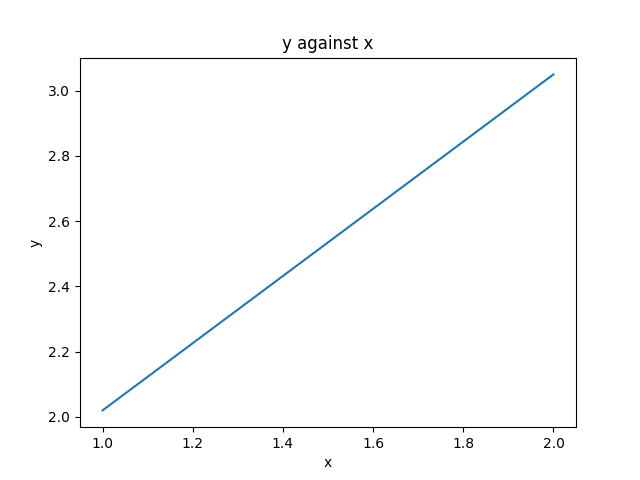
\includegraphics[width=10cm,height=8cm,keepaspectratio]{y against x.png}
    \caption{$y$ against $x$}
    \label{fig:y}
\end{figure}


\begin{table}[H]
    \centering
    \begin{tabular}{|c|c|}
	\hline
	$x$ & $y_{1}$\\
	\hline
	1 & 3\\
	\hline
	2 & 4.\\
	\hline
        
    \end{tabular}
    \caption{$y_{1}$ against $x$}
    \label{tab:$y_{1}$}
\end{table}


\begin{figure}[H]
    \centering
    \includegraphics[width=10cm,height=8cm,keepaspectratio]{y_{1} against x.png}
    \caption{$y_{1}$ against $x$}
    \label{fig:y_{1}}
\end{figure}

\section{Analysis}

\begin{table}[H]
    \centering
    \begin{tabular}{|c|c|}
	\hline
	$y$ & $J_{exp}$\\
	\hline
	2.02 & 368.831\\
	\hline
	3.05 & 369.058\\
	\hline
        
    \end{tabular}
    \caption{$J_{exp}$ against $y$}
    \label{tab:$J_{exp}$}
\end{table}


\begin{figure}[H]
    \centering
    \includegraphics[width=10cm,height=8cm,keepaspectratio]{J_{exp} against y.png}
    \caption{$J_{exp}$ against $y$}
    \label{fig:J_{exp}}
\end{figure}


\begin{table}[H]
    \centering
    \begin{tabular}{|c|c|}
	\hline
	$J_{exp}$ & $z$\\
	\hline
	2.02 & 4.08\\
	\hline
	3.05 & 9.302\\
	\hline
        
    \end{tabular}
    \caption{$z$ against $J_{exp}$}
    \label{tab:$z$}
\end{table}


\begin{figure}[H]
    \centering
    \includegraphics[width=10cm,height=8cm,keepaspectratio]{z against J_{exp}.png}
    \caption{$z$ against $J_{exp}$}
    \label{fig:z}
\end{figure}

\section{Conclusion}

\end{document}
